%!TEX root = main.tex
\section{LWE, SIS, and cryptographic applications}
\label{se:LBC}

%Dans un deuxième temps, Adeline Roux-Langlois définira les problèmes
%{\emph Learning With Errors} (LWE)
%et {\emph Small Integers Solution} (SIS), qui sont au c{\oe}ur de la
%cryptographie
%reposant sur les réseaux euclidiens. Ensuite, elle décrira les chiffrements
%Primal-Regev et Dual-Regev et prouvera leur sécurité à partir du
%problème LWE. Enfin, elle décrira deux familles de signatures reposant
%sur les réseaux euclidiens, dont sont issus les candidats Dilithium et Falcon
%au processus de standardisation du NIST.


To build cryptographic constructions, we need to rely on problems that are always difficult to solve, as the security of a scheme relies on the hardness of an underlying problem. Ideally, we even have a security proof showing that being able to succeed in an attack breaking the scheme is at least as hard as solving an hard problem.

The SVP or CVP problems may be either very hard to solve, either quite easy, depending on the considered lattice. Then we need to define intermediate problems, which are always difficult to solve.
The Short Integer Solution problem and the Learning With Errors problem are two foundamental problems in lattice(based cryptography, they are used to build many constructions from public key encryption scheme and signature schemes to more advanced schemes.


\subsection{Short Integer Solution problem}

The Short Integer Solution problem (SIS) was introduced by Ajtai in 1996. Intuitively, it asks to find a short vector in the lattice $\Lambda^\perp({\bf A}) = \{ {\bf x} \in \mZ^m: {\bf x}^T \cdot {\bf A} = {\bf 0} \bmod q\}$ previously defined in Definition~\ref{def:qary} for an uniformly random matrix ${\bf A} \in \mZ_q^{n \times m}$, where $q$, $n$ and $m$ are integers such that $m \geq n$.
In 1996, Ajtai also showed that finding a short vector in this particular lattice for an uniform $\bf A$ is at least as hard as solving the GapSVP$_{\gamma}$ problem for an approximation factor $\gamma$ polynomial in the dimension $n$ of the lattice.
This reduction is an worst-case to average-case reduction, meaning that solving a problem for an uniform instance (the average case) is at least as hard as solving a problem for all its instances (including the worst one).


\subsubsection{Definition}

\begin{definition}
\label{def:SIS}
The short integer solution problem (SIS$_{q,m,\beta}$) is as follows: given as input a matrix $\bf A$ uniformly chosen in $\mZ_q^{m \times n}$, the goal is to find~${\bf x} \in \mZ^{m}$ such that ${\bf x}^T {\bf A} =  = 0 \bmod q$ and~$0 < \|{\bf x}\| \leq \beta $. 
\end{definition}

The choice of the parameters $n$, $m$, $q$ and $\beta$ is important to be sure the problem is well defined and difficult to solve. Without the condition on the norm of the vector $\bf x$, this problem is easy to solve, it is equivalent to solve an homogeneous system of linear equation.
It admits a solution for any $q$, ${\bf A} \in \mathbb{Z}_q^{m \times n}$ and $\beta \geq \sqrt{m} q^{n/m}$ (Micciancio Regev 2007).

\begin{figure}[h]
\begin{center}

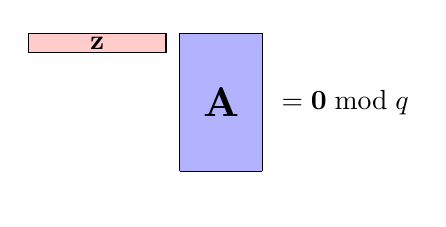
\begin{tikzpicture}[scale=0.35]


\fill[red!20] (-5.5,2.3) rectangle (-0.5,3);
\draw (-5.5,2.3) rectangle (-0.5,3);
\draw (-5.5,2.3) -- (-0.5,2.3);
\draw (-5.5,3) -- (-0.5,3);
\draw (-3,2.65) node {$\bf {z}$};

% Matrice 1
\fill[blue!30] (0,-2) rectangle (3,3) ;
\draw (0,-2) -- (0,3) ;
\draw (3,-2) -- (3,3) ;
\draw (0,-2) -- (3,-2) ;
\draw (0,3) -- (3,3) ;
\draw (1.5,0.5) node[scale=1.5] {$\bf {A}$} ;

\draw (6,0.5) node[scale=1] {$\mathbf{= 0} \bmod q$};

\draw[white] (0,-3) -- (0,-2.8);
\end{tikzpicture} 

\caption{The Short Integer Solution problem.}\label{fig:SIS}
\end{center}
\end{figure}

\paragraph{ISIS.} The ISIS problem is a variant of the SIS problem called the \emph{Inhomogeneous Small Integer Solution} problem. Instead of 
 Au lieu de chercher une solution d'un système homogène, on en cherche une maintenant pour un système d'équations non-homogène.
 
\begin{definition}\label{def:ISIS}
The Inhomogeneous short integer solution problem (SIS$_{q,m,\beta}$) is as follows: given as input a matrix $\bf A$  in $\mZ_q^{m \times n}$, and a vector $\bf{u} \in \mZ_q^n$ both uniformly chosen, the goal is to find~${\bf x} \in \mZ^{m}$ such that~ ${\bf x}^T {\bf A} = {\bf u}^T \bmod q$ and $\|{\bf x}\| \leq \beta $. 

\end{definition}


\subsubsection{Hardness}

In 1996, Ajtai~\cite{Ajtai96} showed that finding a short vector in this particular lattice for an uniform~$\bf A$ is at least as hard as solving the GapSVP$_{\gamma}$ problem for an approximation factor $\gamma$ polynomial in the dimension $n$ of the lattice.
This reduction is an worst-case to average-case reduction, meaning that solving a problem for an uniform instance (the average case) is at least as hard as solving a problem for all its instances (including the worst one). This result is improved in \cite{MR04,GPV08}.



\begin{theorem}[Adapted from~\cite{GPV08}]
\label{th:GPV_SIS}\label{WCAV}
There exists a polynomial time \emph{worst case to average-case} reduction from the \emph{SIVP}$_{\gamma}$ problem to the \emph{SIS}$_{q,m,\beta}$ problem, for any~$m(n), q(n), \beta(n)$ and~$\gamma(n)$ such that $\gamma \geq 2 \beta \sqrt{n}$, $q \geq 2 \beta \sqrt{n}$ and $m,  \log q \leq \text{poly}(n)$.
\end{theorem}


\begin{proof}
We only give the general idea of the proof (and refer to \cite{GPV08} for the full proof), and we simplify it to the case $q = 2 \beta \sqrt{n}$. We also suppose that $\gamma \geq q$ to simplify the reduction, but this condition is not necessary (if $q > \gamma$ we choose $s = \frac{q}{\gamma} \norm{\vec{S}}$).\\


Idea of the reduction: given a basis $\vec{B}$ of a lattice $\Lambda$, we have an oracle which solve SIS, i.e. given a matrix $\vec{A}$ uniform, outputs a short element $\vec{x}$ of norm less than $\beta$ such that  ${\bf x}^T {\bf A} = 0 \bmod q$. The goal is to solve the SIVP problem with an approximation factor $\gamma = 2 \beta \sqrt{n}$.

We use for the reduction a set $\vec{S}$  of linearly independent vectors of the lattice, that we initialize with the basis $\vec{B}$. We then choose a parameter $s =  \norm{\vec{S}} \geq q \cdot  \eta_{\epsilon}(\Lambda)$. 
Note that $\norm{\vec{S}}= \max \norm{\vec{S}_i} \geq \norm{\tilde{\vec{S}}} \geq \eta_{\epsilon}(\Lambda)$, and if $\vec{S}$ is not a solution of SIVP, then $\norm{\vec{S}} \geq \gamma \cdot \lambda_n(\Lambda(\vec{B}))$.\\

The reduction works as follow:
\begin{itemize}
\item Sample $\vec{A}$: for $i=1$ to $m$:
\begin{itemize}
\item $\vec{y}_i \leftarrow D_{\Lambda,s}$ ($\vec{y}_i \in \Lambda$),
\item $\vec{a}_i = \vec{B}^{-1} (\vec{y}_i \bmod q \Lambda) \bmod q \in \mathbb{Z}_q^n$. 
\end{itemize}
We saw that $ \Delta(D_{\Lambda,s,\vec{c}} \bmod \Lambda', U(\Lambda \bmod \Lambda')) \leq 2 \varepsilon$ if $s \geq \eta_{\varepsilon}(\Lambda')$. \\ We have $s \geq q \cdot \eta_{\epsilon}(\Lambda)$ then we have: $ \Delta(D_{\Lambda,s} \bmod q \Lambda, U(\Lambda \bmod q\Lambda)) \leq 2 \varepsilon$ $\Rightarrow$ the $\vec{a}_i$'s are statistically close from uniform in $\mathbb{Z}/ q \mathbb{Z}$. \\
Moreover, the $\vec{y}_i$ 'sare independent, so the $\vec{a}_i$ 'sare too $\Rightarrow$ we can use the SIS oracle.
\item Solving SIS for $\vec{A}$: we obtain nonzero $\vec{z} \in \mathbb{Z}^m$ such that $\vec{z}^T \vec{A} = 0 \bmod q$ and $ 0 < \norm{\vec{z}} \leq \beta$.
\item Combine the elements: let $\vec{x} = \frac{1}{q}\vec{Yz} \in \Lambda$,
\begin{itemize}
\item We first want to show that $\vec{x}$ is an element of the lattice. It suffices to show that $\vec{B}^{-1} \vec{Yz} \in q \mathbb{Z}^m$ (which is equivalent to $\vec{Yz} \in q \Lambda$).  By definition, $\vec{B}^{-1} \vec{Y} = \vec{A} \bmod q$ so $\vec{B}^{-1} \vec{Yz} = \vec{Az} \bmod q = 0 \bmod q$ (it is a solution of the SIS problem).
\item  We have $\norm{\vec{Yz}}  \leq s \beta \sqrt{n}$ then $\norm{\vec{x}} \leq s/2$ $\Rightarrow$ it's a shorter element!
\end{itemize}
To solve SIVP, we repeat this procedure several times to obtain a new set on répète cette procédure plusieurs fois pour obtenir un nouvel ensemble $\vec{S}'$ tel que $\norm{\vec{S}} \leq \norm{\vec{S}'} / 2$. \\
Cette réduction fonctionne aussi pour le problème ISIS en ajoutant un centre bien choisi aux Gaussiennes pour les $\vec{y}_i$.
\end{itemize}
\end{proof}


\subsubsection{Application: hash function}

\begin{definition}
Let $m \geq 4 n \log q$, for a matrix $\vec{A} \in \mathbb{Z}_q^{m \times n}$, we define $f_{\vec{A}} : \{0,1\}^m \rightarrow \mathbb{Z}_q^n$ by:
$$ f_{\vec{A}} (\vec{x}) = \vec{x}^T \vec{A} \bmod q.$$
\end{definition}


We start with an important lemma, which shows that for any input $\vec{x}$, the output $ \vec{x}^T \vec{A}$ is statistically indistinguishable from a uniform element in $\mZ_q^{n}$, knowing $\vec{A}$. It is called a Leftover Hash Lemma.

\begin{lemma}
\label{le:LHL}
Let $m, n, q \ge 1$ be integers such that $m \geq 4 n \log q$ and $q$ is prime, and let $\vec{A} \hookleftarrow U(\mZ_q^{m \times n})$ and $\vec{r} \hookleftarrow U(\{0,1\}^m)$. Then the statistical distance between $(\vec{A},\vec{r}^T \vec{A})$ and the uniform distribution on $\mZ_q^{m \times n} \times \mZ_q^{n}$ is less than $\leq 2^{-n}$.
\end{lemma}

The condition  $m \geq 4 n \log q$ is important, it allows sufficient entropy.



\begin{theorem}
\label{th:resistanceCollision}
If the SIS problem is difficult to solve for $\beta \geq \sqrt{m}$, then the Ajtai's hash function is collision resistant.
\end{theorem}

\subsection{Learning With Errors problem}

The LWE problem was introduced by Regev in 2005~\cite{Reg05}. Intuitively, it asks to solve a BDD instance (see Definition~\ref{def:BDD}) in the following lattice $ \Lambda_q(\vec{A}) = \{ \vec{y} \in \mathbb{Z}^m : \vec{y} =\vec{As} \bmod q \text{ for } \vec{s} \in \mathbb{Z}^n\},$ previously defined in Definition~\ref{def:qary} for an uniformly random matrix ${\bf A} \in \mZ_q^{n \times m}$, where $q$, $n$ and $m$ are integers such that $m \geq n$.




\subsubsection{Definition}

The computational variant of LWE asks to find a vector $\vec{s} \in \mZ_q^n$ given an arbitrary number of noisy scalar product between $\vec{s}$ and some known $\vec{a}_i$'s uniformly chosen in $\mZ_q^n$. Its decisional variant asks to distinguish those noisy scalar products from uniform elements.

\begin{definition}
Let $n \geq 1$, $q\geq 2$ prime, and $\alpha \in ]0,1[$. The distribution $D^{\mbox{\tiny LWE}}_{n,q,\alpha}(\vec{s})$ is a distribution on
$\mZ_q^{n+1}$ obtained with the following experiment: 
\begin{itemize}
\item sample $\vec{a} \hookleftarrow U(\mZ_q^n)$,
\item sample $e \hookleftarrow D_{\mZ,\alpha q}$,
\item Output $(\vec{a}, \ps{\vec{a}}{\vec{s}} +  e \bmod q )$.
\end{itemize}
The Learning with Errors problem is defined as follow:
\begin{itemize}
\item Search variant of LWE$_{n,q,\alpha}$: Let $\vec{s} \leftarrow U(\mZ_q^{n})$, given an arbitrary number of samples from $D^{\mbox{\tiny LWE}}_{n,q,\alpha}(\vec{s})$, find $\vec{s}$.
\item Decisional variant of LWE$_{n,q,\alpha}$: Let $\vec{s}\hookleftarrow U(\mZ_q^{n})$,  distinguish between the distributions $D^{\mbox{\tiny LWE}}_{n,q,\alpha}(\vec{s})$ and $U(\mZ_q^{n} \times \mZ_q)$.
\end{itemize}
\end{definition}

Usually, the parameter $q$ is chosen polynomial in $n$ and $\alpha$ is chosen between $1/q$ and $q$.
The choice of $\alpha$ is important here, if it is too small, the noise of each sample can be zero with high probability and then it is easy to find $\vec{s}$. If $\alpha$ is too large, then $e$ can be close to be uniformly distributed modulo~$q$. The distribution $D^{\mbox{\tiny LWE}}_{n,q,\alpha}(\vec{s})$ will be too close from uniform and independant from $\vec{s}$ and then it will be impossible to find $\vec{s}$.




\subsubsection{Reduction from search to decision}

Regev~\cite{Reg05} showed an important result on the equivalence of the two version of LWE.

\begin{lemma}
The two LWE variants, search and decisional, are computationally equivalent.
\end{lemma}

It is an interesting property as search problems are usually harder than decision ones, but in security proofs we often rely on a decisional problem. The first direction of the reduction is quite direct since if we are able to solve the search problem, the resulting secret would allow to distinguish between an LWE distribution and a uniform one.


\begin{proof}
Suppose that an algorithm $\mathcal{A}$ can efficiently solve the decisional variant of LWE, we will use it to solve the search variant.
We start by solving this variant with a non negligible probability on $\vec{s} \hookleftarrow U(\mZ_q^n)$. 
We have access to an oracle sampling from $D^{\mbox{\tiny LWE}}_{n,q,\alpha}(\vec{s})$, and to $\mathcal{A}$, 
and we want to find $\vec{s}$. Let's show how to find the first coordinate $s_1$ 
of~$\vec{s}$. As $q$ is small, one can try all the possible values $s_1^*$ of~$s_1$, and then use~$\mathcal{A}$ to validate this value. Using a sample $(\vec{a},b)= (\vec{a}, \ps{\vec{a}}{\vec{s}} + e)$, 
we give to $\mathcal{A}$ the following input 
\[(\vec{a},b)+ (u,0,\ldots,0, u s_1^*) = (\vec{a}', \ps{\vec{a}'}{\vec{s}} + e + u (s_1^*-s_1)), \ 
\mbox{avec} \ u \hookleftarrow U(\mZ_q).
\]
Then:
\begin{itemize}
\item if $s_1^* = s_1$, the input sample given to $\mathcal{A}$ is following the
$D^{\mbox{\tiny LWE}}_{n,q,\alpha}(\vec{s})$ distribution;
\item if $s_1^* \neq  s_1$, then the last coordinate is uniformly distributed and independent from the $n$ other, as $u$ is uniform and $s_1^*-s_1$ invertible modulo~$q$.
\end{itemize}   
The answer of $\mathcal{A}$ tells us if the guess~$s_1$ for is correct.

If it is possible to find $\vec{s}$ with a non-negligible probability, when $\vec{s} \hookleftarrow U(\mZ_q^n)$, then it is possible for any $\vec{s}$.
Indeed, for a fixed $\vec{s}$, we can sample $\vec{t} \hookleftarrow U(\mZ_q^{n})$, and transform the sample $(\vec{a},\ps{\vec{a}}{\vec{s}} + e)$ of $D^{\mbox{\tiny LWE}}_{n,q,\alpha}(\vec{s})$ in a sample $(\vec{a},\ps{\vec{a}}{\vec{s} + \vec{t}} + e)$ of $D^{\mbox{\tiny LWE}}_{n,q,\alpha}(\vec{s}+\vec{t})$.
As $\vec{s}+\vec{t}$ is uniform, we can find $\vec{s}+\vec{t}$, and then~$\vec{s}$.
\end{proof}

This first reduction is provided only for~$q$ prime and $\text{poly}(n)$, but for any error distribution. It also needs $m' = \tilde{O}(nmq/\varepsilon^2)$ search LWE samples to call the decision oracle with $m$ samples, where $\varepsilon$ is the advantage of the oracle to distinguish between the two distributions. 
The conditions on the parameters of this reduction (in particular on $q$) was later improved in several works~\cite{Pei09,MP12,BLPRS13}, but only for Gaussian distributions, and with a similar loss on the number of samples.
There also exists a sample-preserving search-to-decision reduction given by Micciancio and Mol~\cite{MM11}, this reduction only works for particular cases, as for instance $q$ prime and $\text{poly}(n)$ for any discrete error on $\mZ_q$.


\subsubsection{Hardness of LWE}



\paragraph{Quantum reduction.} Regev~\cite{Reg05,Reg09} was the first to provide a worst-case to average-case reduction showing the hardness of the Learning With Errors problem. This reduction has the particularity to use a quantum algorithm. This mean given an oracle to solve LWE, we only have a quantum algorithm to solve Approx-GapSVP. Then, if it happens that an attacker can solve LWE, he will need a quantum computer to polynomially solve Approx-GapSVP or SIVP for all possible instances (i.e. even in the worst-case). 

\begin{theorem}[{\cite[Th. 1.1]{Reg05}}]
Let $q >2$ and $\alpha \in (0,1)$ be function of $n$ such that $\alpha q \geq 2 \sqrt{n}$. If $q$ is prime and polynomial in $n$, then there exists a worst-case to average-case quantum polynomial time reduction from \emph{GapSVP}$_{\gamma}$ (or \emph{SIVP}$_{\gamma}$) in dimension~$n$ to \emph{LWE}$_{n,q,\alpha}$ for $\gamma = \tilde{O}(n/\alpha)$. 
\end{theorem}


\paragraph{High level idea of Regev's proof.} We refer to~\cite{Reg05} for the full proof. 
Regev defines an intermediate problem called DGS (discrete Gaussian sampling problem):


\begin{itemize}
\item DGS$_{\phi}$: given a lattice $\Lambda$ of dimension $n$ and a parameter $r > \phi(\Lambda)$. Output a sample of $D_{\Lambda,r}$.
\end{itemize}
Remark: the hardness of this problem depends on the basis of $\Lambda$ that we have. Then the smaller is $r$, the harder it is to solve.
Then Regev described two reductions:

\medskip

%\lecours{\textcolor{blue}{

\begin{itemize}
\item A reduction from SIVP with $\gamma=\tilde{O}(n / \alpha)$ to DGS with $r=2 \sqrt{n} \eta_{\varepsilon}(\Lambda) / \alpha$.
\begin{itemize}
\item Principle of the reduction from SIVP$_{2\sqrt{n} \phi(L)}$ to DGS$_{\phi(L)}$ if $\phi(L) \geq 2  \eta_{\varepsilon}(L)$:
\begin{itemize}
\item Given a lattice $L$, we start by using LLL to obtain $S$ = set of $n$ vectors linearly independent of size at most $2^n \lambda_n(L)$. We denote by $\tilde{\lambda}_n$ the norm of the largest, by construction $\lambda_n(L) \leq \tilde{\lambda}_n \leq 2^n \lambda_n(L) $.
\item For $i \in \{0, \ldots, 2n \}$, call DGS $n^2$ times on $(L,r_i = \tilde{\lambda}_n 2^{-i})$ to build the set $S_i$. (check if $r_i > \phi(L)$)
\item Choose the $n$ vectors linéairement linearly independent in each $S_i$ and output the shortest set.
\end{itemize}
\item Why does it work?
\begin{itemize}
\item If $\phi(L) \geq \tilde{\lambda}_n $, $S$ is already smaller than $2 \sqrt{n} \phi(L)$.
\item Else, let $i$ such that $\phi(L) < r_i < 2 \phi (L)$ (exists because $\lambda_n(L) \leq \tilde{\lambda}_n \leq 2^n \lambda_n(L) $, $\phi(L) \geq 2  \eta_{\varepsilon}(L)$ and $\eta_{\varepsilon}(L) \geq \lambda_n(L)/n$). There are  $n$ vectors linearly independent in $S_i$ with high probability (see Corollary 3.16 Regev 09). All the vectors of $S_i$ has norm at most $\sqrt{n} r_i \leq 2 \sqrt{n} \phi (L)$.
\end{itemize}
\end{itemize}
\item If $\alpha q > 2 \sqrt{n}$, a quantum reduction from DGS for $r= \sqrt{2n} \eta_{\varepsilon}(\Lambda) / \alpha$ to LWE$_{q,\alpha}$.
\begin{itemize}
\item Input : a lattice $L$ and $r > 2 \sqrt{n} \eta_{\varepsilon}(\Lambda) / \alpha$. Goal: a sample from $D_{L,r}$.
\item Principle: two iterations. Let $r_i = r \cdot (\alpha q / \sqrt{n})^i$. The algorithm starts by producing $n^c$ samples of $D_{L,r_{3n}} $ (he can do it because $r_{3n} > 2^{3n}r > 2^{2n} \lambda_n(L)$). Iteration:
\begin{itemize}
\item Classical step: given $n^c$ samples of $D_{L,r_i}$ and an LWE oracle, solve CVP$_{L^*,\frac{\alpha q}{r}}$ (variant where the distance between the target and the lattice is $\frac{\alpha q}{r}$). 
\item Quantum step: use the CVP$_{L^*,\frac{\alpha q}{r}}$ oracle to find $n^c$ samples of $D_{L,r_{i-1}}$.
\end{itemize}
\item At the end, we have $n^c$ samples of $D_{L,r_0}$ with $r_0=r$.
%$r_ 1 =r \cdot \alpha q / \sqrt{n} > \sqrt{2} q \eta_{\varepsilon}(\Lambda) $
\end{itemize}
\end{itemize}
%}


\paragraph{Classical reductions.} In 2009, Peikert~\cite{Pei09} gave the first classical reduction to show the hardness of the LWE problem, but his result was limited to an exponential modulus $q$ in the dimension $n$. Compared to the original reduction of Regev, this reduction is also limited to GapSVP.

\begin{theorem}[{\cite[Th. 3.1]{Pei09}}]
Let $q >2$ and $\alpha \in (0,1)$ be function of $n$, there exists a worst-case to average-case classical polynomial time reduction from \emph{GapSVP}$_{\gamma}$ in dimension~$n$ to \emph{LWE}$_{n,q,\alpha}$ for $\gamma \geq \frac{n}{\alpha \log n}$ and $q \geq 2^{n/2} \cdot \omega(\sqrt{\log n /n})$. 
\end{theorem}

\paragraph{Classical hardness for a polynomial modulus.} In 2013~\cite{BLPRS13}, Brakerski \emph{et al.} provided a classical reduction to show the hardness of the Learning With Errors problem, for a polynomial modulus $q$ in the dimension $n$. This smaller size of the modulus is the one used in practice, this reduction also remove the condition on~$q$ to be prime.

\begin{theorem}[{\cite{BLPRS13}}]
Let $q >2$ and $\alpha \in (0,1)$ be function of $n$ such that $\alpha q \geq \sqrt{n}$. There exists a worst-case to average-case classical polynomial time reduction from \emph{GapSVP}$_{\gamma}$ in dimension~$\sqrt{n}$ to \emph{LWE}$_{n,q,\alpha}$ for $\gamma = \tilde{O}(n^2/\alpha)$. 
\end{theorem}

The main idea of this reduction is to start from Peikert's result, i.e. a classical reduction from GapSVP to LWE for an exponential modulus. And then to use a modulus switching technique to provide a reduction from LWE with an exponential modulus to LWE with a polynomial modulus, at the expense of making the error term grows. 
 Note than an important step for this reduction to work is to use LWE with a smaller secret.
Overall, this reduction looses a factor $\sqrt{n}$ in the dimension of the two problems, if we compare to Regev's quantum reduction.
Those results can be summarised in Table~\ref{tab:LWE}.

\begin{table}[h]
\begin{center}
\begin{tabular}{c|c|c|c|c|c}
%\hline
& dim $n'$ & $q$ & $\alpha$ & $\gamma$ & \\
\hline
\cite{Reg05} & $n$ & $\text{poly}(n)$, prime  & $\alpha q \geq 2\sqrt{n}$& $\tilde{O}(n/\alpha)$ & quantum \\[0.3em]
\cite{Pei09} & $n$ & $q> 2^{n/2}$ & $\alpha q \geq n$ & $ \geq n /(\alpha \log n)$ & classical \\[0.3em]
\cite{BLPRS13} & $\sqrt{n}$ & $\text{poly}(n)$ & $\alpha q \geq \sqrt{n}$ & $\tilde{O}(n^2/\alpha)$ & classical \\
%\hline
\end{tabular}
\caption{Reductions from GapSVP$_{n', \gamma}$ to LWE$_{n,q,\alpha}$.}
\label{tab:LWE}
\end{center}
\end{table}

Finally, an important consequence of the work of~\cite{BLPRS13} is to show that the hardness of LWE in dimension $n$ and with a modulus $q$ is a function of $n \log q$. This is shown by the modulus switching reduction which gives a reduction from LWE$_{n,q}$ to LWE$_{n/k,q^k}$ and from LWE$_{n,q^k}$ to LWE$_{nk,q}$.







%}


\paragraph{Other variants}


\subsection{Public Key encryption scheme on LWE}

\subsubsection{Regev's encryption scheme}

\subsubsection{Dual Regev encryption scheme}


\subsection{Signature scheme}

\subsubsection{Signature using Fiat Shamir transformation}

\subsubsection{Trapdoors and GPV signature scheme}